% !TeX spellcheck = en_US
\chapter{The Proposed Decentralized Solution}\label{cha:decentralizedSystem}

This chapter describes the proposed centralized solution used to answer the four questions presented in the problem statement (\cref{sec:problemStatement}). The expectation supporting this thesis is that the decentralized solution will perform better than the centralized solution (presented in \cref{cha:existingSystem}) on the following parameters:

\begin{description}
	\item[Availability] in terms of fault tolerance. Decentralizing the Park Pilot out on the turbines removes the Park Pilot as a single point of failure. Thus the decentralized solution should be able to handle the situation where a the situation where a turbine fails.
	\item[Performance] in terms of regulation cycle time. Having all data needed, in order to perform the regulation, available locally on every turbine, thus enabling every turbine to regulate themselves, removes the time spent requesting data and waiting for replies from the regulation cycle.
	\item[Scalability] in terms of turbines per Park Pilot, which ultimately controls the regulation cycle time. The cycle time is controlled by the worst case number of turbines per Park Pilot (i.e. worst case state retrieval time, worst case new setpoint calculations, worst case time it takes to broadcast new setpoints). Thus the theory is that decentralizing the Park Pilot would enable a more dynamic system, where increasing the number of turbines also increases the resources (in terms of CPU power and RAM) available to the Park Pilot, but also increases the number of packages on the network to the point where the network bandwidth becomes inadequate. Siemens has informed that the current Siemens solution operates on a gigabit network, making network bandwidth a small issue, but an issue that has to be solved at some point nevertheless. Even when this issue presents itself, one could imagine a decentralized system where the turbines are automatically clustered, where one cluster represents a Park Pilot, in order to decrease number of receivers per turbine, thus decreasing the number of packages on the network.
\end{description}


\noindent The decentralized solution is built using the knowledge of the current Siemens system, obtained when developing the centralized solution. Thus changes made from the centralized solution to the decentralized solution are only specific to the change in the architecture when decentralizing the system, meaning QoS parameters, that does not get in the way of decentralizing the system, and data sent and received is the same for both systems.

This chapter describes the decentralized solution by first describing what decentralizing the system means to the regulation algorithm. Furthermore the chapter describing the decentralized solution through a detailed description of the regulation cycle of the decentralized solution, followed by a description of the DDS QoS parameters used. 

\section{Regulation algorithm}

Decentralizing the regulation algorithm from the centralized solution (\cref{sec:cenRegAlgorithm}), we get the input/outputs presented on \cref{fig:ioDecenRegAlg}.

\begin{figure}
	\centering
	\begin{tikzpicture}[
	point/.style={inner sep=0pt}, %circle,minimum size=2pt,fill=red},
	textNode/.style={inner sep=2pt},
	hv path/.style={to path={-| (\tikztotarget)}},
	vh path/.style={to path={|- (\tikztotarget)}},
	skip loop h/.style={to path={-- ++(0,#1) -| (\tikztotarget)}},
	skip loop v/.style={to path={-- ++(#1,0) |- (\tikztotarget)}},
	graphs/every graph/.style={edges=rounded corners}
	]
	
% Place nodes
\matrix[row sep=1.5cm,column sep=.5cm] {
	\node [point]  		(p1x1)	{}; &&
	\node [rectangle]	(Turbine)		[draw, label=above:Turbine, text width=50pt]	{Cur.prod. Max.prod}; &&
	\node [point]  		(p1x3)	{}; \\
	
	\node [point]  		(p2x1)			{}; &&
	\node [textNode]	(HPPP)		 	{Reg.algorithm}; &&
	\node [textNode]	(Setpoint)	{Setpoint}; \\

	\node [textNode]  (gSetpoint)										{Global setpoint}; &&
	\node [rectangle]	(Data)			[draw, text width=50pt] {Cur.prod  Max.prod};\\
};

\node [textNode,right of=Data] {~~~~~~~~~~~~~~~~~\textbf{$\cdot$}nTurbines-1};
	
\graph[use existing nodes]{
	Turbine ->[skip loop v=-3.1cm] HPPP -> Setpoint ->[vh path] Turbine;
	gSetpoint.east -> HPPP;
	Data -> HPPP;
};

\end{tikzpicture}

	\captionsetup{format=plain,font=footnotesize,labelfont={bf,defaultCapFont},labelsep=quad,singlelinecheck=no}
	\caption[Decentralized input/output parameters of the regulation algorithm]{
		\label{fig:ioDecenRegAlg} 
		\footnotesize{%
			Decentralized input/output parameters of the regulation algorithm.
		}
	}
\end{figure}

The regulation algorithm is now computed on every turbine instead of computing the algorithm on an external Park Pilot. Thus, instead of getting all states (current production and max production) externally, the regulation algorithm now gets one state from the local turbine. Furthermore the regulation algorithm now only calculates a single setpoint - the setpoint used by the local turbine to set a new state - instead of calculating a setpoint for every turbine in the wind farm.

As \cref{fig:ioDecenRegAlg} implies, with the regulation algorithm performed on every turbine, decentralizing the Park Park onto the turbines also means that every turbine now needs the state of every other turbine in the wind farm.



\section{Regulation cycle}

Decentralizing the Park Pilot onto the turbines also means a change in the regulation cycle. The decentralized solution has been built with focus on scalability, in terms of increasing the number of turbines does not impact the regulation cycle, and performance, in terms of decreasing the regulation cycle time.

The following sections describes the decentralized regulation cycle. First by presenting how the decentralized regulation cycle differs from the centralized regulation cycle through, followed by a detailed description of how a single regulation cycle has been implemented. 

%Finally the term \textit{cache reads} is discussed, which is introduced by the decentralized by a discussion of the introduction of cache reads.

\subsection{Changes from the centralized regulation cycle}

The difference between the centralized regulation cycle and the decentralized regulation cycle is illustrated on \cref{fig:cycleCentralVSDecentral}. 

\begin{figure}
	%The figure show how regulation time differs central vs decantral

	{\sffamily{Centralized regulation cycle}}
	\newline
	

{ %The brackets issolate the enviroment

\tikzstyle{line}		 	= [draw]

\makeatletter
\ifcsname c@wavenum\endcsname %Only create one counter
\else
	\newcounter{wavenum}
\fi
\makeatother

\newcommand*{\bitvector}[3]{
  \draw[fill=#3] (t_cur) -- ++( .1, .3) -- ++(#2-.2,0) -- ++(.1, -.3)
                         -- ++(-.1,-.3) -- ++(.2-#2,0) -- cycle;
  \path (t_cur) -- node[anchor=mid](textNode) {#1} ++(#2,0) node[time] (t_cur) {};
  }

% \known{val}{length}
\newcommand*{\known}[2]{
    \bitvector{#1}{#2}{white}
}

% \unknown{length}
\newcommand*{\unknown}[2]{
    \bitvector{#1}{#2}{black!20}
}

% \nextwave{name}
\newcommand{\nextwave}[1]{
  %\path (0,\value{wavenum}) node[time] (t_cur) {};
   \path (0,\value{wavenum}) node[left] {#1} node[time] (t_cur) {};
  \addtocounter{wavenum}{-1}
}

\newcommand{\timeSpanLabel}{
	\node (CycleTimeLabel) [rectangle, above = 0.7cm of textNode, inner sep=0pt] {Regulation cycle time};	  
}

\newcommand{\timeSpanA}{
	\node (t_timeSpanA) [point, above = 0 of t_cur] {};	  
}

\newcommand{\timeSpanB}{
	\node (t_timeSpanB) [point, above =0 of t_cur] {};

  \graph[use existing nodes]{
  	t_timeSpanA --[time span=1cm] CycleTimeLabel;
   	CycleTimeLabel.south --[time span=-0.24cm] t_timeSpanB;
  }; 
    	
}


%%% End of timing.sty
\begin{tikzpicture}[
	point/.style={inner sep=0pt}, %circle,minimum size=2pt,fill=red},
	draw=black, 
	yscale=.8,
	xscale=1,
	hv path/.style={to path={-| (\tikztotarget)}},
	vh path/.style={to path={|- (\tikztotarget)}},
	skip loop v/.style={to path={-- ++(#1,0) |- (\tikztotarget)}},		
	skip loop h/.style={to path={-- ++(0,#1) -| (\tikztotarget)}},
	time span/.style={to path={-- ++(0,#1) -| (\tikztotarget)}},
	graphs/every graph/.style={edges=rounded corners}	
	]
	
  \tikzstyle{time}=[coordinate]
  \setlength{\unitlength}{1cm}
  \setcounter{wavenum}{0}
    
  %\nextwave{Regulation Time} \unknown{SendData}{2} \known{WaitForData}{5} \unknown{ReciveData}{2} \unknown{Calculate}{2}\unknown{SendSP}{2}
  \nextwave{Park Pilot} \unknown{reqStates}{1.8} \known{wait}{2} \unknown{readStates}{2} \unknown{regAlg.}{1.7} \unknown{sendSetpoints}{2.6}
  
  \nextwave{Turbine} \known{wait}{1.8} \unknown{replyState}{2} \known{wait}{6.3} \unknown{receiveSetpoint}{2.9}
    
  
\end{tikzpicture}
}

	\newline
	
	{\sffamily{Decentralized regulation cycle (with parallel reception of data)}}
	\newline
	

{ %The brackets issolate the enviroment

\makeatletter
\ifcsname c@wavenum\endcsname %Only create one counter
\else
	\newcounter{wavenum}
\fi
\makeatother

\newcommand*{\bitvector}[3]{
  \draw[fill=#3] (t_cur) -- ++( .1, .3) -- ++(#2-.2,0) -- ++(.1, -.3)
                         -- ++(-.1,-.3) -- ++(.2-#2,0) -- cycle;
  \path (t_cur) -- node[anchor=mid](textNode) {#1} ++(#2,0) node[time] (t_cur) {};
}

% \known{val}{length}
\newcommand*{\known}[2]{
    \bitvector{#1}{#2}{white}
}

% \unknown{length}
\newcommand*{\unknown}[2]{
    \bitvector{#1}{#2}{black!20}
}

% \nextwave{name}
\newcommand{\nextwave}[1]{
  %\path (0,\value{wavenum}) node[left] {#1} node[time] (t_cur) {};
  %\path (0,\value{wavenum}) node[time] (t_cur) {};
  \path (0,\value{wavenum}) node[below left] {#1} node[time] (t_cur) {};
  \addtocounter{wavenum}{-1}
}


\newcommand{\timeSpanA}{
	\node (t_timeSpanA) [point, above = 0 of t_cur] {};	  
}

\newcommand{\timeSpanB}{
	\node (t_timeSpanB) [point, above =0 of t_cur] {};
	
	\graph[use existing nodes]{
		t_timeSpanA --[time span=1cm] CycleTimeLabel;
		CycleTimeLabel.south --[time span=-0.24cm] t_timeSpanB;
	}; 
	
}

%%% End of timing.sty

\begin{tikzpicture}[
	point/.style={inner sep=0pt}, %circle,minimum size=2pt,fill=red},
	draw=black, 
	yscale=.8,
	xscale=1,
	hv path/.style={to path={-| (\tikztotarget)}},
	vh path/.style={to path={|- (\tikztotarget)}},
	skip loop v/.style={to path={-- ++(#1,0) |- (\tikztotarget)}},		
	skip loop h/.style={to path={-- ++(0,#1) -| (\tikztotarget)}},
	time span/.style={to path={-- ++(0,#1) -| (\tikztotarget)}},
	graphs/every graph/.style={edges=rounded corners}	
]
	
\tikzstyle{time}=[coordinate]
\setlength{\unitlength}{1cm}
\setcounter{wavenum}{0}

	\nextwave{Turbine} \unknown{readStates}{2.5} \unknown{regAlg.}{2.5} \unknown{setSetpoint}{2.5} \unknown{sendState}{2.5} \known{sleep}{2}
	\nextwave{} \known{reciveStates}{12}
\end{tikzpicture}
}

	\caption{Centralized vs decentralized regulation cycle}
	\label{fig:cycleCentralVSDecentral}
\end{figure}

Where a request for data and waiting for the corresponding reply for every turbine was needed for the Park Pilot in the centralized solution, turbines now publishes new states whenever a new setpoint has been calculated. Turbines publishes to a specific \textit{Topic} and are assigned a unique \textit{key}. Receiving states from other turbines is then handled and loaded asynchronously into memory by \textit{Connext}, thus making receiving states happen in parallel with the regulation algorithm. This enables \textit{Distributed Shared Memory (DSM)} (see \cref{sec:DSM} for \textit{DSM} description) behavior for the decentralized solution, where the state of every turbine is shared with every other turbine in the wind farm. Since every turbine has a unique \textit{Topic key}, each turbine has assigned its own shared memory space, where only the turbine is allowed to write, as illustrated on \cref{fig:DSMlikeBehavior}, thus removing the possibility that turbines overwrite each others states. Using \textit{DSM} like behavior for the decentralized solution, means that receiving states from other turbines is abstracted away from the regulation cycle, enabling the turbines to assume that the latest state of every other turbine has been received and is available locally in memory, thus removing the need for the request-reply part of the centralized regulation cycle. The expectation is that removing the request-reply part of the algorithm decreases the regulation cycle time, since acquisition of turbines states are no longer a part of the cycle.  

\begin{figure}
	\begin{tabular}{ | c | c | c | c | c |}
		\cline{1-3}
		\cline{5-5}
		turbine 1 & turbine 2 & turbine 3 & \dots & turbine n \\
		\cline{1-3}
		\cline{5-5}
	\end{tabular}
	\caption{Distributed Shared Memory like behavior of the decentralized solution}
	\label{fig:DSMlikeBehavior}
\end{figure}

Removing the request-reply part of the regulation cycle for the decentralized solution, also removes the ability to ensure that regulation happens using latest states only, since a given turbine, when initiating the regulation cycle, reads the turbine states that is already in memory, instead of requesting all the latest states. This of cause forces a redefinition of when a state is usable for regulation. Instead of using latest states only, the decentralized solution defines a time limit that, when reached, changes the status of the state to old and thus not usable for regulation. Thus for the decentralized solution it is acceptable to perform regulation using states that are no older than the specified time limits. 

To further decrease the regulation cycle time, strictly reliable messaging has been removed for the decentralized solution. A reply from all turbines at a specific point in the regulation cycle is no longer needed, thus package losses will no longer block the regulation cycle. Furthermore, with the time limit introduced, all states are no longer needed by every turbine, since states now only have to be strictly 'younger' than the specified time limit. Therefore to further reduce the regulation cycle, strictly reliable messaging has been removed. Instead, for the decentralized solution, best effort messaging, where data samples are sent once and missed samples are acceptable, has been used. This introduces determinism to the regulation cycle by removing potential communication delays, thus reducing the regulation cycle time. This also means that every turbine of the decentralized solution is only interested in the newest published state and not every state published, meaning a dropped state are overwritten by the state of the next regulation cycle for a given turbine.

Each turbine only calculates its own setpoint. Thus after calculation, the new setpoint is set locally and the new state is published to the other turbines. The wait in the end is there to leave a small amount of time for \textit{Connext} to receive and overwrite states that have already been read.

\subsection{Implementation}

Before running the cycle illustrated on \cref{fig:decenRegCycle}, an initial setpoint is set and the corresponding state of the turbine is read, enabling publishing the turbine state as the first step of the regulation cycle. This is done to prevent the first cycle from being redundant due to lack of data from other turbines. 

\begin{figure}
	\centering
	\begin{sequencediagram} %Created using pgf-umlsd
		\newthread{parkPilot}{:Park Pilot}
		\newinst[2]{turbine}{:Turbine}
		\newinst[2]{connext}{:Connext}
		
		\begin {messcall}{parkPilot}{publishState()}{connext}{}
		\end {messcall}
		\begin {call}{parkPilot}{readStates()}{connext}{states}
		\end {call}
		\begin {callself}{parkPilot}{regAlgorithm()}{setpoint}
		\end {callself}
		\begin {call}{parkPilot}{sendSetpoint()}{turbine}{setpoint}
		\end {call}
		\begin {call}{parkPilot}{readState()}{turbine}{state}
		\end {call}	
		\begin {callself}{parkPilot}{sleep()}{}
		\end {callself}			
	\end{sequencediagram}

	\captionsetup{format=plain,font=footnotesize,labelfont={bf,defaultCapFont},labelsep=quad,singlelinecheck=no}
	\caption[Decentralized regulation cycle sequence diagram]{
		\label{fig:decenRegCycle} 
		\footnotesize{%
			Decentralized regulation cycle sequence diagram.
		}
	}
\end{figure}

\Cref{fig:decenRegCycle} presents three objects:

\begin{itemize}
	\item The \textbf{Park Pilot} object which handles the regulation cycle. As opposed to the centralized solution, the Park Pilot object is now instantiated on every turbine in the wind farm, instead of being a single external component.
	\item The \textbf{Turbine} object which serves as the interface to the underlying Turbine. The Turbine object for the purpose of this thesis is just a simulation of an actual turbine. Thus this object handles communication with a database with actual turbine data provided by Siemens.
	\item \textit{Connext} is the underlying DDS framework used for communication, thus this is not an object instantiated by the Park Pilot. It is however what enables reception of data in parallel with the regulation cycle. 
\end{itemize}

The Park Pilot publishes the state of the present turbine and reads the states of every turbine within the wind farm. Afterwards the regulation algorithm is performed and a setpoint for the present turbine is calculated and used to set a new state.

The regulation algorithm used for the decentralized solution is the same used for the centralized solution described in \cref{sec:calculateSetpoints}.

\subsection{Cache reads}

A cache read happens if the cycle time elapses before all turbine instances have responded with state information, resulting in the same state being read twice. Thus it is a natural result of separating receiving data from the regulation cycle, as done in the decentralized solution. \textit{Connext} only keeps track of data that has already been read but not how many times that data has been read. Thus a cache read does not include information regarding if the same state has been read multiple times.

The regulation cycle of the decentralized solution does not directly include any communication, thus enabling a significant reduction of regulation cycle time. However, decreasing the cycle time, increases the 'pressure' on \textit{Connext} by increasing the number of regulation cycles pr. minute, thus increasing the number of states that needs to be published, thus increasing the number of states that needs to be received (assuming that the cycle time of all turbines are equally decreased). This ultimately results increased number of cache reads and increased network traffic. Thus reducing the regulation cycle time is expected to increase the number of cache reads.  

Increasing the number of cache reads can be an issue, since it reduces the effectiveness of the regulation cycle. Having a high number of cache reads implies that the regulation has been performed using data used for the previous regulation, thus decreasing the effect of the current regulation.

As a result of this trade-off between reduction in regulation cycle time and number of cache reads, a sleep in the end of the regulation cycle (as presented on \cref{fig:decenRegCycle}) has been implemented, in order to control the reduction of the regulation cycle. Thus the regulation cycle time is an input parameter of the decentralized solution.

\section{DDS configuration} \label{sec:decen:ddsconf}

\begin{figure}
\begin{lstlisting}[language=XML]
<participant_factory_qos>
    <logging>
        <verbosity>WARNING</verbosity>
        <category>PLATFORM</category>
        <print_format>VERBOSE_TIMESTAMPED</print_format>
        <output_file>ddsadaptor.log</output_file>
    </logging>
</participant_factory_qos>
\end{lstlisting}
\caption[Decentralized participant factory QoS parameters]{
		\label{fig:decParFacQos} 
		\footnotesize{Participant factory QoS parameters of the decentralized solution.}
	}
\end{figure}

\section{Graphical Interface} \label{sec:graphicalInterface}
In order to visualize the system a graphical user interface has been constructed using Matlab, Simulink and DDS Blockset for Simulink.
These tools combined allows the creation of a Simulink model which taps into the communication of the DDS framework.
The data collected from via the Simulink model can then be transferred to Matlab for further processing or visualization.

The main objective of the graphical interface is to visualize what messages is currently flowing in the system but almost as important is the ability to collect data for further analysis.
Matlab is a powerful tool for anlysis and having the data transferred live from the DDS framework to matlab allows for both live as well as in depth analysis on a dataset collected during an experiment.

Currently only the decentralized system can be visualized and controlled using the graphical interface. Given the scope and focus of this thesis the value added by visualizing the centralised system would be minimal. Both the decentralized and centralized system can log data using the Simulink models.

\subsection{DDS Blockset for Simulink}
RTI has created a Blockset for Simulink allowing a Simulink model to interact with the DDS Participant and other entities in a DDS enabled network.
The blockset consists of a toolbox containing 6 blocks. Common for all blocks except the DDS Time block is that they can be configured with a default or custom Quality of Service profile as well as a sample time. The Quality of Service profile must match the profile used in the network you want to participate in. The sample time is related to the Simulink model and specifies the timeinterval between samples.

\begin{figure}[h]
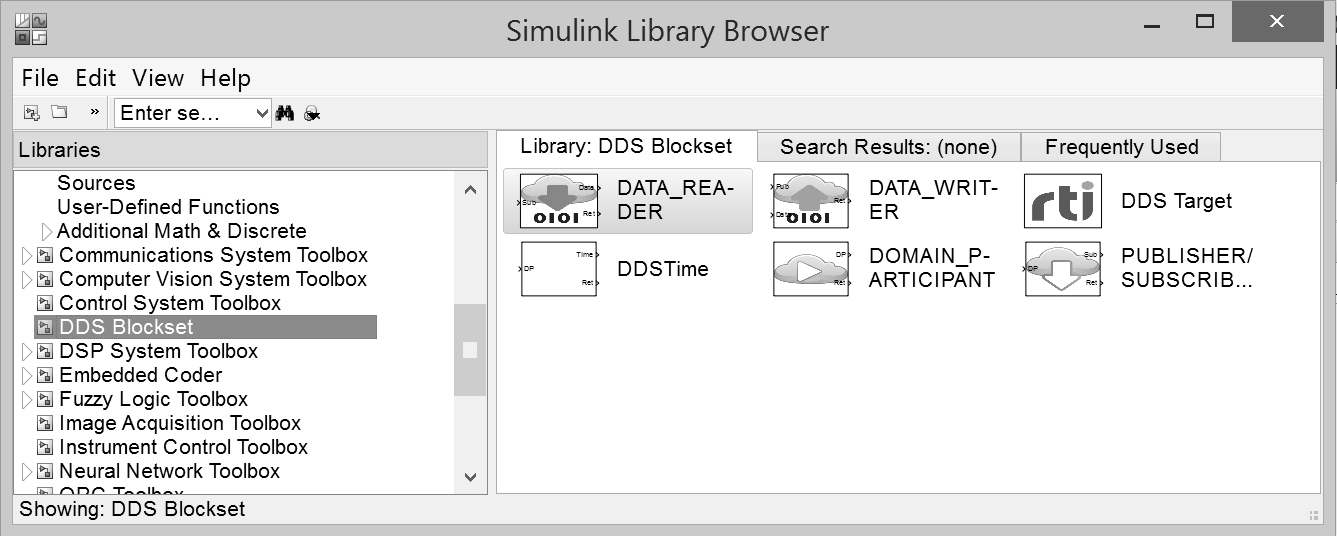
\includegraphics[width=\textwidth]{figures/DDSBlockset}
\captionsetup{format=plain,font=footnotesize,labelfont={bf,defaultCapFont},labelsep=quad,singlelinecheck=no}
	\caption[DDSBlockset blocks for Simulink]{
		\label{fig:DDSBlocksetBlocks} 
		\footnotesize{%
			DDSBlockset blocks for Simulink.
		}
	}
\end{figure}


\paragraph{The DomainParticipant block} is the equivalent to the DomainParticipant entity in DDS. This block allows for configuration of the DomainID which links the DomainParticipant to a specific DDS domain.

\paragraph{The Publisher/Subscriber block} can be configured as either a Publisher or a Subscriber and will act as either based on the chosen configuration.

\paragraph{The DataWriter block} is the equivalent to the DataWriter entity in DDS. This block can write data to a topic in DDS. The DataWriter block must be configured with the name of the Topic as well as the name of the Topic Type created by the Simulink Bus that is input to the DataWriter.

\paragraph{The DataReader block} is the equivalent to the DataReader entity in DDS. This block can read data from a topic in DDS. The DataReader block must be configured with the name of the Topic as well as the name of the Topic Type created by the Simulink Bus that is input to the DataReader. The DataReader block can also be configured to either use Read() or Take() for obtaining the DDS data. The Read() command will leave the data in DDS memory, the Take() command will remove the data from DDS memory. The DataReader block is able to either poll DDS for data or wait for data until data is ready or a timeout occurs.

\paragraph{The DDSTarget block} is controls code generated for the DDS blocks in the Simulink model. It is possible to configure which version of DDS code will be generated for, either RTI Connext DDS(default), or RTI Connext Micro DDS. The type system can be configured to either static or dynamic as well as the discovery mode.

\paragraph{The Time block} can return the current time from DDS output in seconds and nanoseconds.

\subsection{Installation of DDS Blockset for Simulink}
To install DDS Blockset for Simulink follow the steps provided by Mathworks \cite{DDSBlocksetPilotSupportPackageUserGuide}. The installation is short but as described below additional work had to be done in order to make DDS Blockset for Simulink work properly with Matlab and Interface Definition Language files.

The problems described in the section all relates to installation of DDS Blockset for Simulink using Matlab 2013b on a Windows 8.1 x64 environment.
Other environments may be more or less optimal but have not been tested during this thesis.

There are a few caveats to be avoided when installing DDS Blockset for Simulink on Windows.
After installation of DDSBlockset for Simulink completes make sure the NDDSHOME path variable is set to \path{C:\ Program Files(x86)\ RTI}.
Notice that this path is different from the default path recommended by RTI which is \path{C:\ Program Files(x86)\ RTI\ ndds.5.0.0} (version numbers may change).

DDS Blockset for Simulink has an import feature available for import of Interface Definition Language files. The import process creates a Simulink bus that the Simulink model can hook into and pull data from. In order to enable import of Interface Definition Language files additional setup must be performed.
Since Matlab does not provide a compiler fro C++ on x64 systems one must be downloaded. Microsoft provides a compiler in the Microsoft Windows SDK 7.1. Matlab must be told to use the compiler by using the mex -setup command. Finally the location of the binaries and the libraries that is downloaded with the new compiler must be added to path.

\subsection{Simulink model of the decentralized system}\label{subsec:decentralizedmodel}

\begin{figure}[b]
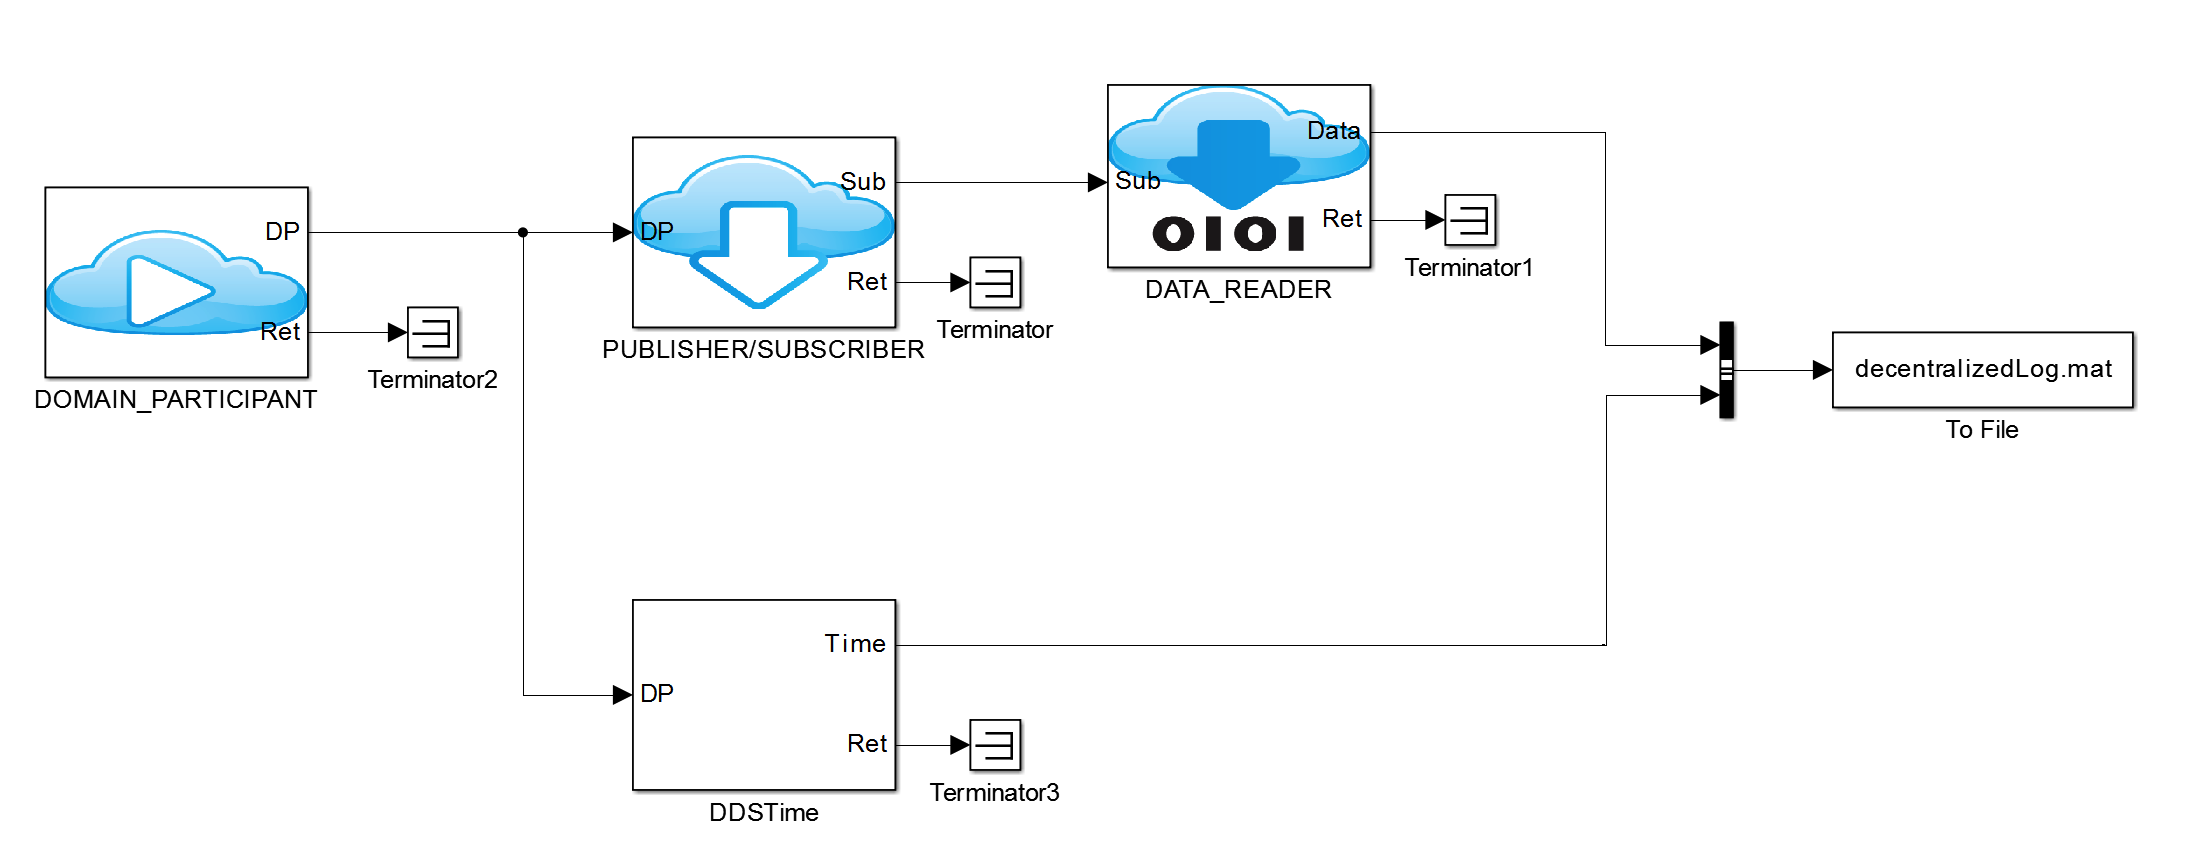
\includegraphics[width=\textwidth]{figures/DecentralizedModel}
\captionsetup{format=plain,font=footnotesize,labelfont={bf,defaultCapFont},labelsep=quad,singlelinecheck=no}
	\caption[Decentralized Simulink model]{
		\label{fig:decentralizedSimulinkModel} 
		\footnotesize{%
			Decentralized Simulink model.
		}
	}
\end{figure}

The Simulink model of the decentralized system is simple. The decentralized Simulink model has a DomainParticipant block in order to be able to receive data from the same domain as the turbines. It also has a Time block to enable logging and graphing of the current DDS time. Since the decentralized system only uses one DDS message type, TurbineMessage \{INSERT REFERENCE\}, to communicate between all the turbines in the system, the decentralized Simulink model has only one Subscriber block and one DataReader block. The Subscriber block specifies the topic to subscribe to and the DataReader block receives events every time a new TurbineMessage is available. The TurbineMessage that is received is logged to a .mat file together with the current DDS time for later use.

In order to transfer data from the Simulink model to Matlab eventlisteners must be implemented in a Matlab .m file. In the decentralized system the eventhandler listens for incoming events on the bus object that receives new data from the DataReader block. When new data is received the event fires and data can be collected from the Simulink model. Furthermore model execution can be controlled from Matlab, as well as parameters like model runtime.

\subsection{Simulink model of the centralized system}\label{subsec:centralizedmodel}
The Simulink model of the centralized system is a bit more complex. The centralized system contains three different messagetypes, TurbineDataMessage, RequestMessage, SetpointMessage, \{INSERT REFRENCE\} that all run on different topics. Because of this the centralized Simulink model contains one DomainParticipant, three Subscribers, one for each topic, and three DataReaders, one for each message type, in order to capture the communication in the centralized system. Every message received is logged to a .mat file together with the current DDS time.

\begin{figure}[h]
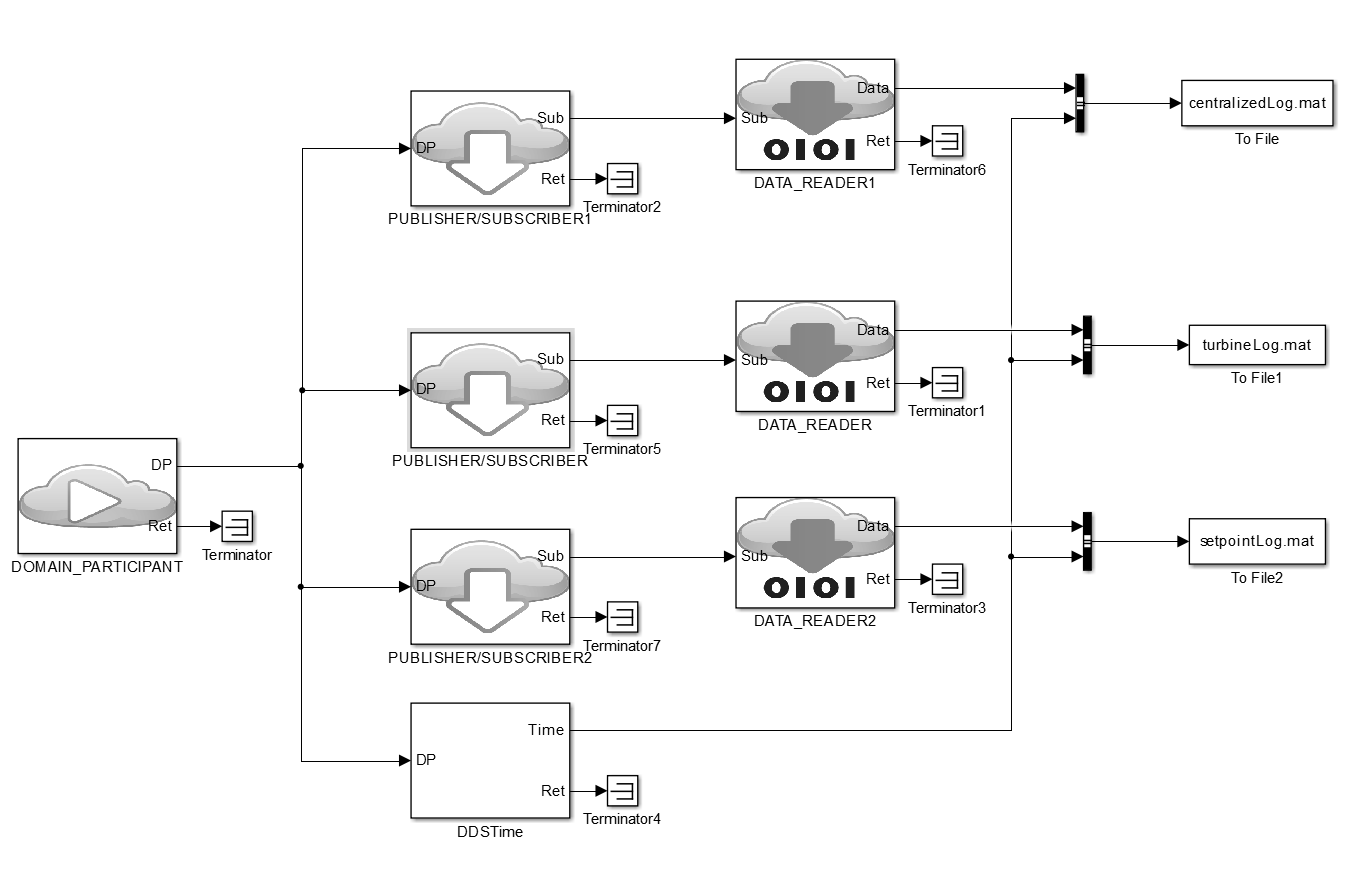
\includegraphics[width=\textwidth]{figures/CentralizedModel}
\captionsetup{format=plain,font=footnotesize,labelfont={bf,defaultCapFont},labelsep=quad,singlelinecheck=no}
	\caption[Centralized Simulink model]{
		\label{fig:centralizedSimulinkModel} 
		\footnotesize{%
			Centralized Simulink model.
		}
	}
\end{figure}